\documentclass[aspectratio=1610]{beamer}
%\documentclass[aspectratio=1610, handout]{beamer}
\usepackage[utf8]{inputenc}
\usepackage{ragged2e}
\usepackage{xcolor}
\usepackage[italian]{babel}
\usepackage{multirow}
\usetheme[progressbar=frametitle,titleformat=smallcaps]{metropolis}
\setbeamertemplate{frame numbering}[fraction]
\setbeamercovered{dynamic}
\definecolor{rosso}{RGB}{255, 0, 0}
\definecolor{giallo}{RGB}{254,212,23}
\hypersetup{colorlinks=true,linkcolor=black,urlcolor=rosso}
\setbeamercolor{palette primary}{fg=black, bg=giallo}
\setbeamercolor{background canvas}{bg=white}
\setbeamercolor{normal text}{fg=black}
\setbeamercolor{progress bar}{fg=rosso}
\setbeamercolor{framesubtitle}{fg=rosso}
\setbeamercolor{normal text .dimmed}{fg=giallo}
\setbeamercolor{block title alerted}{fg=rosso, bg=giallo}
\setbeamerfont{caption}{size=\tiny}
\setbeamerfont{caption name}{size=\tiny}
\setlength{\abovecaptionskip}{0pt}
\makeatletter
\metroset{block=fill}
\setlength{\metropolis@progressinheadfoot@linewidth}{1pt} 
\setlength{\metropolis@progressonsectionpage@linewidth}{1pt}
\setlength{\metropolis@titleseparator@linewidth}{1pt}
\makeatother

\title{CRITTOGRAFIA}
\subtitle{https, cifrari a chiave simmetrica}
\date{}
\institute{\textit{
        Fonti:
        \begin{itemize}
            \item[-] \href{https://www.treccani.it/enciclopedia/crittografia\_(Enciclopedia-della-Scienza-e-della-Tecnica)/}{Treccani}
            \item[-] \href{https://it.wikipedia.org/wiki/Storia\_della\_crittografia}{Wikipedia}
        \end{itemize}
    }
}

\begin{document}

\begin{frame}[plain, noframenumbering]
    \titlepage
\end{frame}

\section{CRITTOGRAFIA}

\begin{frame}{CRITTOGRAFIA}
    \begin{alertblock}{DEFINIZIONE}
        \begin{minipage}{0.98\linewidth}
            \justifying
            La crittografia è la disciplina che studia le \textbf{tecniche per trasformare un messaggio, 
            detto testo in chiaro, in un altro messaggio, detto testo cifrato, che risulta incomprensibile} 
            a chiunque non conosca tutti i dettagli della tecnica usata per la trasformazione. 
            Solo il legittimo destinatario del messaggio è in grado di effettuare l’operazione inversa 
            e di ottenere così dal testo cifrato il testo in chiaro originale. La trasformazione del testo 
            in chiaro in testo cifrato è detta \textbf{cifratura}, mentre la ricostruzione del testo in chiaro 
            a partire dal testo cifrato è detta \textbf{decifratura}. L’insieme delle operazioni che devono 
            essere effettuate durante la cifratura e la corrispondente decifratura prende il nome di codice 
            crittografico, o \textbf{cifrario}.\\
            \bigskip
            \tiny{\textbf{Curiosità}}\\
            \tiny{\href{https://it.wikipedia.org/wiki/Crittografia_end-to-end}{Crittografia end-to-end}}
        \end{minipage}
    \end{alertblock}
\end{frame}

\begin{frame}{HTTP vs HTTPS}
    \begin{columns}
        \column{.5\textwidth}
            \begin{figure}
                \href{http://www.flowgorithm.org/}{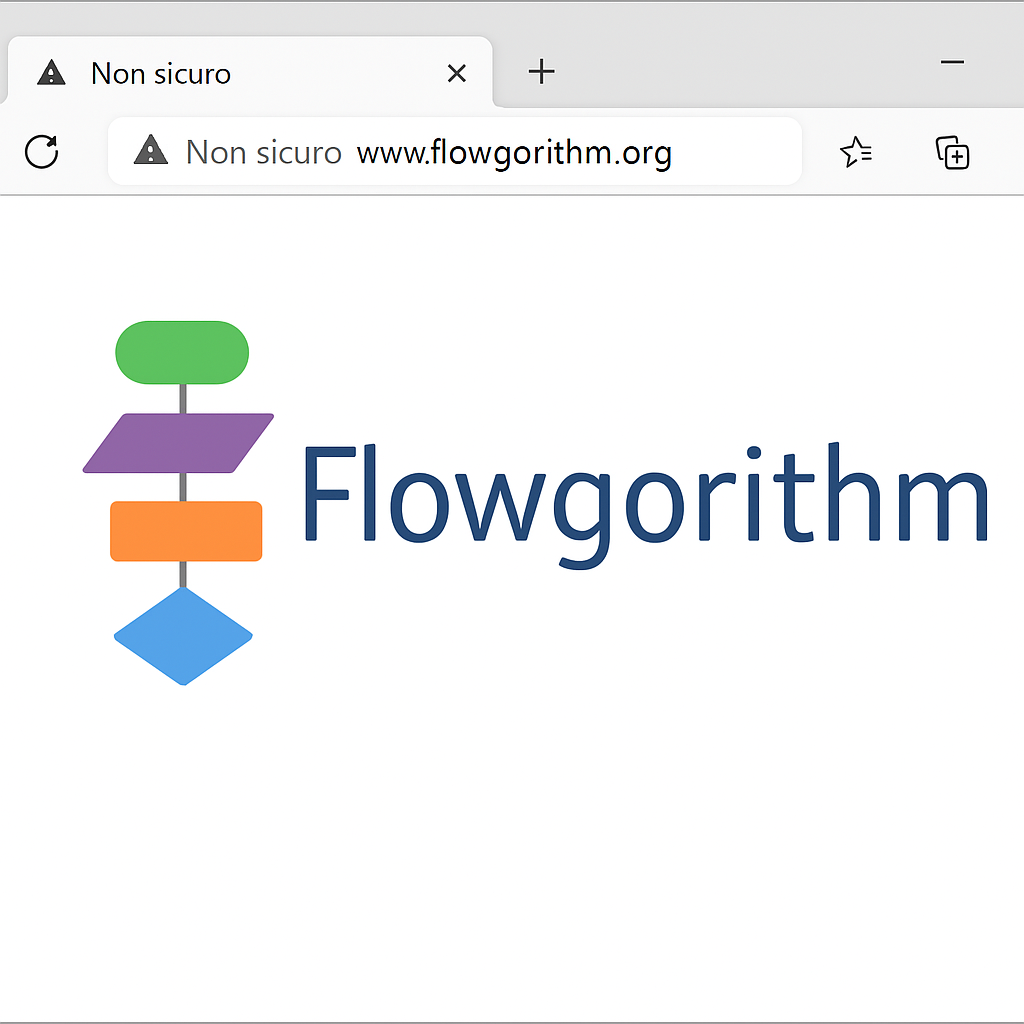
\includegraphics[width=\linewidth]{img/flowgorithm.png}}
                \caption{{creata con \href{https://chatgpt.com/}{ChatGPT}}}
            \end{figure}
        \column{.5\textwidth}
            \begin{figure}
                \href{https://www.netflix.com/it/}{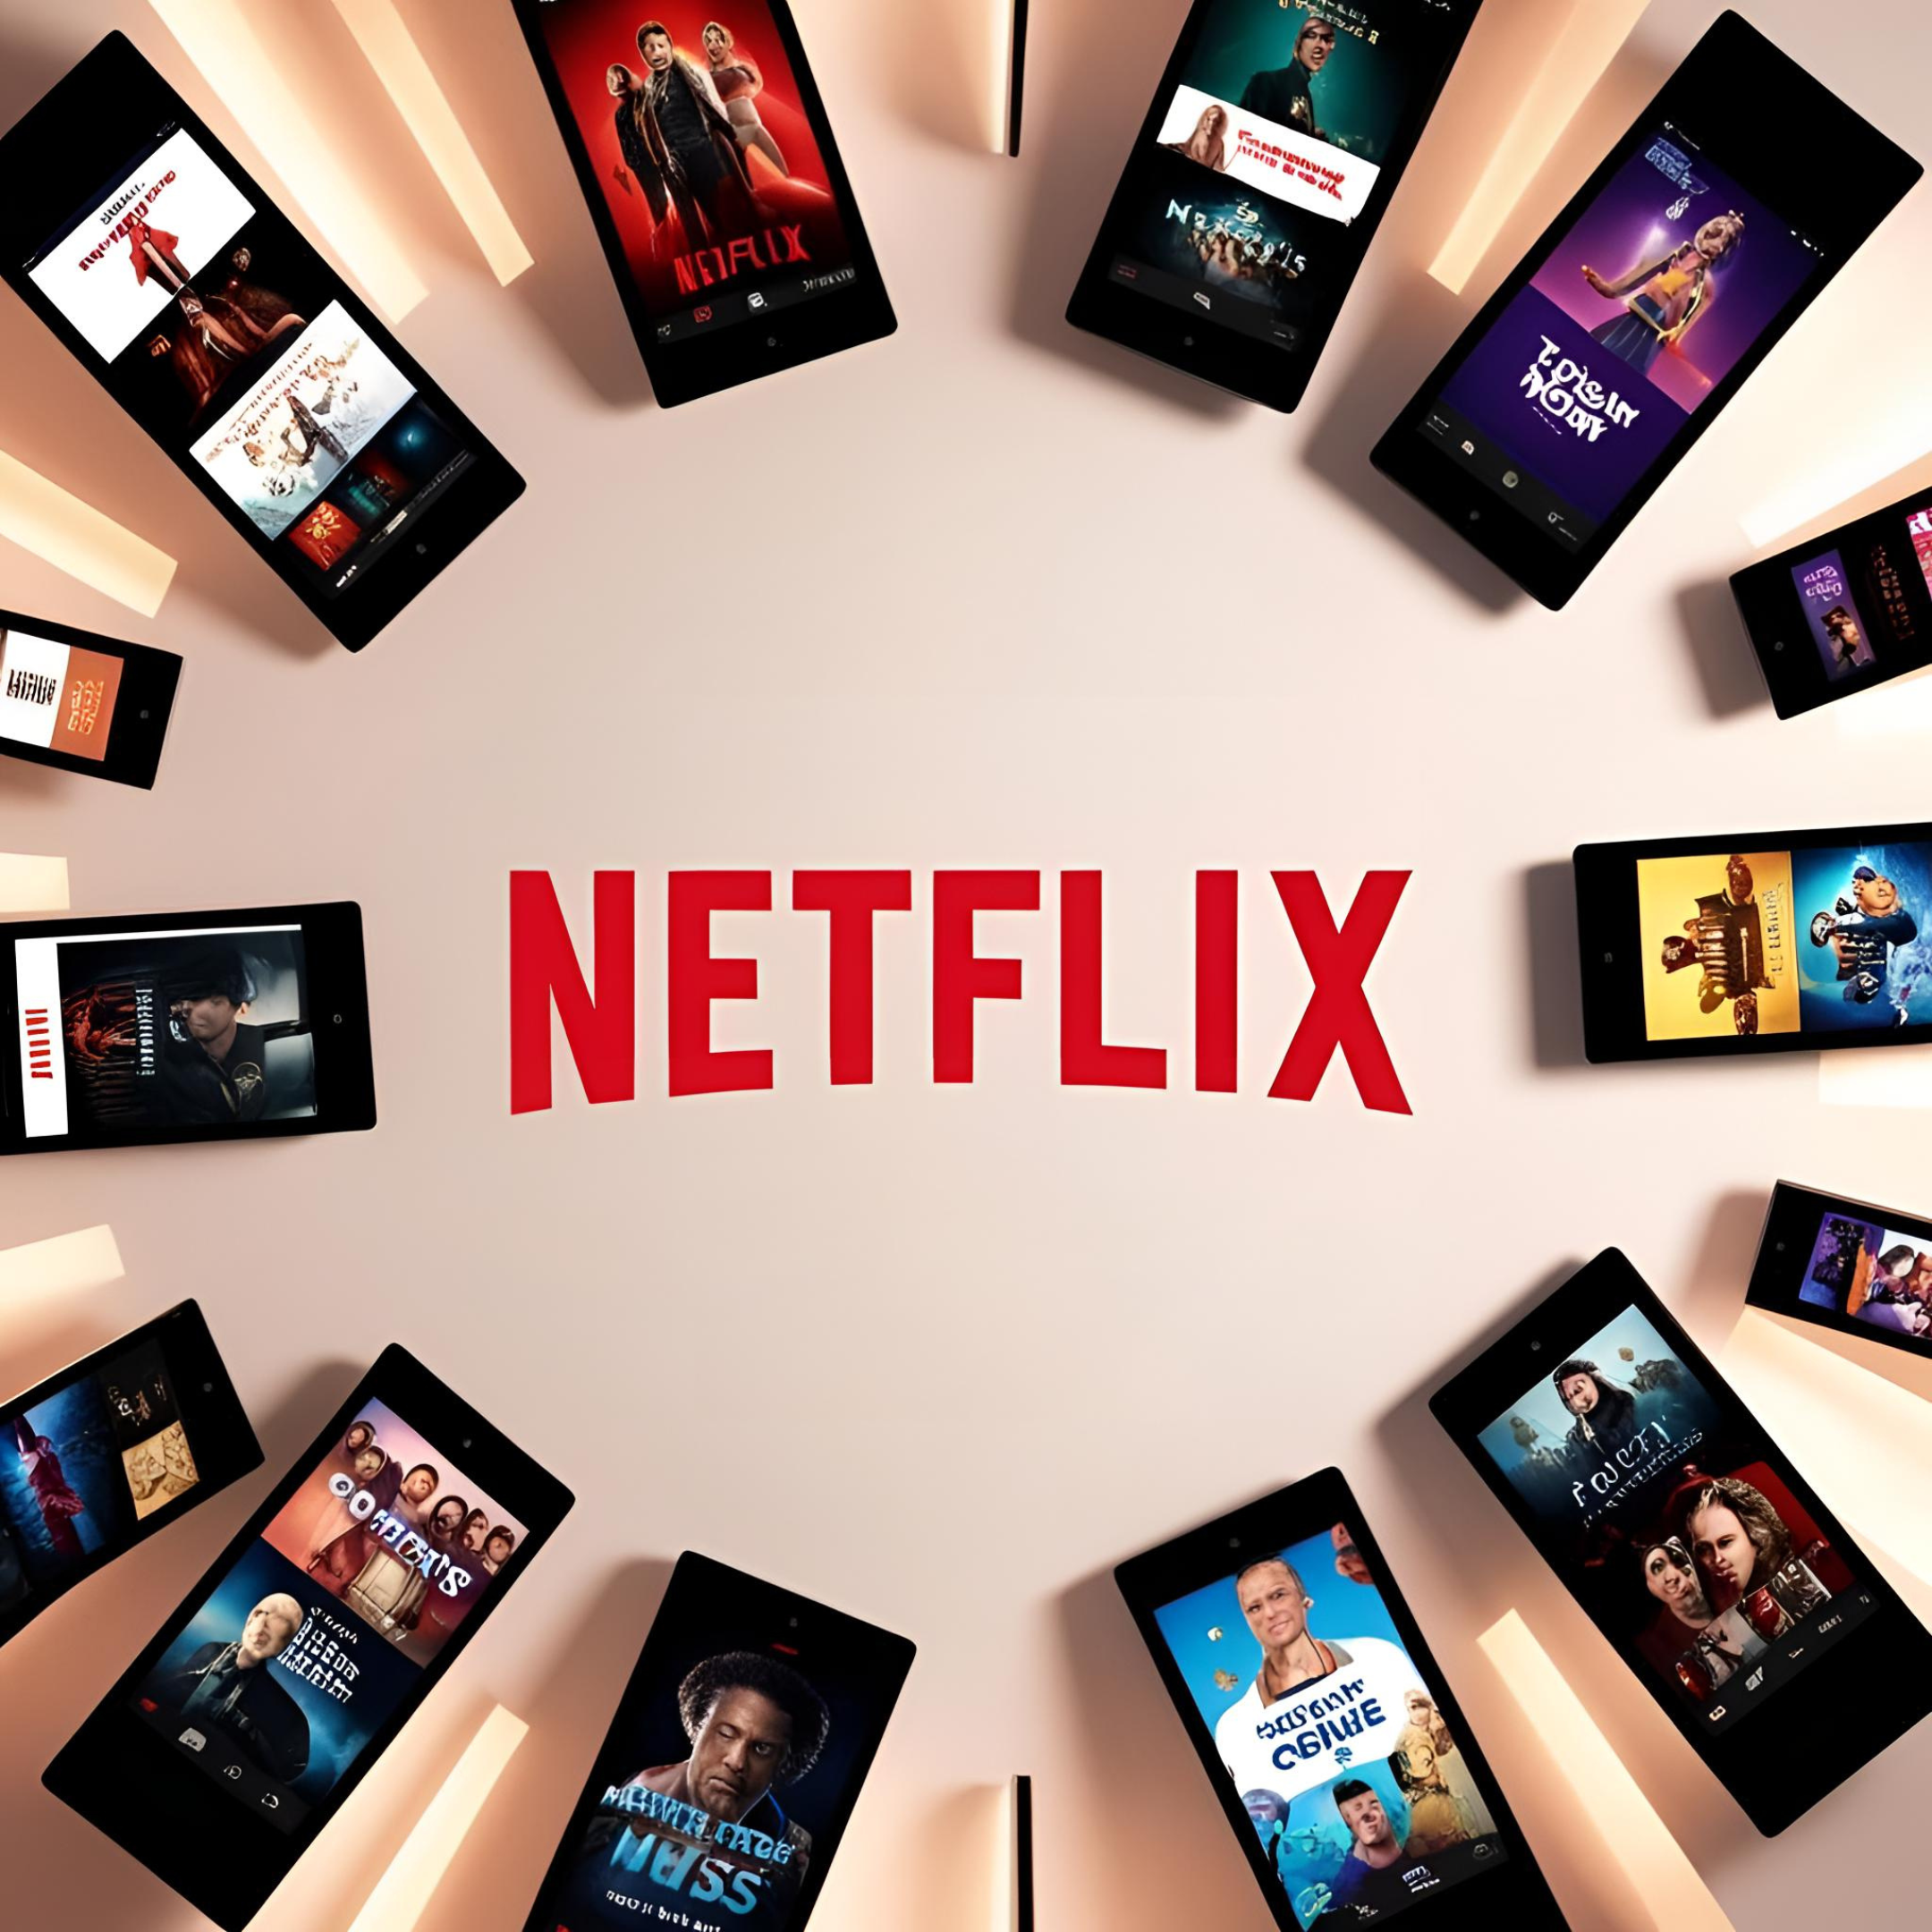
\includegraphics[width=\linewidth]{img/netflix.png}}
                \caption{{creata con \href{https://www.canva.com/}{Canva}}}
            \end{figure}
    \end{columns}
\end{frame}

\section{CIFRARI SIMMETRICI}

\begin{frame}{CIFRARIO DI CESARE}
    \begin{alertblock}{DEFINIZIONE}
        \begin{minipage}{0.98\linewidth}
            \justifying
            Il cifrario di Cesare è uno dei più antichi algoritmi crittografici di cui si abbia traccia storica. 
            È un cifrario a \textbf{sostituzione monoalfabetica, in cui ogni lettera del testo in chiaro è sostituita, 
            nel testo cifrato, dalla lettera che si trova un certo numero di posizioni dopo nell'alfabeto}. 
            (nel caso del cifrario di Cesare, il numero di posizioni è 3). Questi tipi di cifrari sono detti anche 
            cifrari a sostituzione o cifrari a scorrimento a causa del loro modo di operare: la sostituzione avviene 
            lettera per lettera, scorrendo il testo dall'inizio alla fine.\\
            \bigskip
            \tiny{\textbf{Esempio}}\\
            \tiny{\href{http://www.crittologia.eu/critto/caesar.html}{Cifrario di Cesare}}
        \end{minipage}
    \end{alertblock}
\end{frame}

\begin{frame}{CIFRARIO DI VERNAM (OTP)}
    \begin{alertblock}{DEFINIZIONE}
        \begin{minipage}{0.98\linewidth}
            \justifying
            Esempio di cifrario a \textbf{chiave non riutilizzabile}, in inglese \textbf{One Time Pad} abbreviato in \textbf{OTP}. 
            Il cifrario di Vernam è perfetto, nel senso che il testo in chiaro e il testo cifrato sono del tutto indipendenti, 
            la conoscenza dell'uno non dà alcuna informazione sull'altro. È quindi del tutto al sicuro dagli attacchi della crittanalisi statistica. 
            \textbf{La chiave utilizzata per cifrare il messaggio deve essere lunga quanto il messaggio stesso} e non deve 
            essere mai riutilizzata, per questo viene chiamata One Time Password. Per ottenere il testo cifrato è sufficiente 
            eseguire un'operazione di \href{https://it.wikipedia.org/wiki/Disgiunzione\_esclusiva}{XOR} tra il testo in chiaro 
            e la chiave.\\
            \bigskip
            \tiny{\textbf{Esempio}}\\
            \tiny{\href{http://www.crittologia.eu/critto/vernam.phtml}{Cifrario OTP}}
        \end{minipage}
    \end{alertblock}
\end{frame}

\end{document}